\documentclass[UTF8,a4paper,12pt]{ctexart}

\usepackage{amsmath,amssymb}
\usepackage{booktabs}
\usepackage{caption}
\usepackage{float}
\usepackage{geometry}
\usepackage{graphicx}
\usepackage{hyperref}
\usepackage{longtable}
\usepackage{xcolor}
\usepackage{enumitem}
\usepackage{fvextra}

\geometry{left=2.6cm,right=2.6cm,top=2.6cm,bottom=2.6cm}
\hypersetup{colorlinks=true,linkcolor=black,urlcolor=blue}
\setlength{\parindent}{2em}
\setlength{\parskip}{0.25em}
\setlength{\emergencystretch}{3em}
\sloppy
\linespread{1.25}
\setlist[itemize]{leftmargin=2.5em,itemsep=0.15em}
\DefineVerbatimEnvironment{CodeBlock}{Verbatim}{breaklines,breakanywhere,fontsize=\small,frame=single,rulecolor=\color{gray!45}}

\title{\heiti 机器学习与Python实践\\[0.8em]\Large 第五次作业\\[1.6em]\Huge 基于Auto数据集的汽车款式聚类分析}
\author{}
\date{}

\begin{document}

\begin{titlepage}
    \centering
    \vspace*{1.2cm}
    
\includegraphics[width=0.78\linewidth]{figures/cover_logo.png}\par
    \vspace{1.0cm}
    {\zihao{2}\heiti 机器学习与Python实践\par}
    \vspace{0.8cm}
    {\zihao{3}\heiti 第五次作业\par}
    \vspace{1.2cm}
    {\zihao{1}\heiti 基于Auto数据集的汽车款式聚类分析\par}
    \vfill
    \begin{tabular}{rl}
        姓名：& 匿名\\[0.45em]
        专业：& 强基班\\[0.45em]
        学号：& \\[0.45em]
        教师：& 匿名\\[0.45em]
        学院：& 信息科学与工程学院\\[0.45em]
    \end{tabular}
    \vfill
    {\zihao{4}2026年6月15日\par}
\end{titlepage}

\tableofcontents
\newpage

\section{前言及问题概述}

汽车市场中的车型在燃油经济性、发动机规格、整车重量、动力性能和生产年代等方面存在明显差异。面对大量车型参数，消费者往往难以仅凭单个指标判断车辆之间的相似性。聚类分析能够在没有人工类别标签的情况下，根据样本间的特征距离自动发现数据内部结构，将参数相近的汽车划分到同一组，为车型定位、市场细分和购车比较提供参考。

本次实验使用题目给出的 ISLR \texttt{Auto} 数据集。数据集共包含 392 辆汽车和 8 个特征，分别为每加仑汽油可行驶英里数 \texttt{mpg}、气缸数 \texttt{cylinders}、发动机排量 \texttt{displacement}、发动机马力 \texttt{horsepower}、重量 \texttt{weight}、从 0 加速至 60 mph 所需时间 \texttt{acceleration}、生产年份 \texttt{year} 和生产地 \texttt{origin}。其中 \texttt{origin} 的取值 1、2、3 分别表示美国、欧洲和日本。

题目要求根据汽车参数进行聚类，识别相似汽车。本实验属于无监督学习任务，不存在预先给定的真实类别。实验首先完成数据质量检查和探索性分析，再对连续变量进行标准化、对生产地进行 One-Hot 编码；随后扫描不同聚类数，使用肘部法、轮廓系数、Calinski--Harabasz 指数和 Davies--Bouldin 指数选择合理的聚类数；最后比较 K-Means、Ward 层次聚类、Gaussian Mixture 和 DBSCAN，并通过 PCA 降维图、轮廓图和聚类画像解释汽车款式差异。

\section{相关基础知识及方法}

\subsection{相关原理}

聚类的目标是在没有类别标签的条件下，将样本集合划分为若干组，使同一组内的样本尽可能相似，不同组之间的样本尽可能不同。设第 $i$ 辆汽车的特征向量为 $x_i$，聚类结果为 $c_i\in\{1,\ldots,K\}$，则聚类算法需要根据特征空间中的距离或概率分布确定 $c_i$。

K-Means 是最常用的划分式聚类方法。给定聚类数 $K$，算法通过反复执行“分配样本”和“更新中心”两个步骤，最小化簇内平方和：
\begin{equation}
    J=\sum_{k=1}^{K}\sum_{x_i\in C_k}\left\|x_i-\mu_k\right\|_2^2,
\end{equation}
其中 $C_k$ 表示第 $k$ 个簇，$\mu_k$ 为该簇的中心。K-Means 计算速度快、结果容易解释，但需要预先指定 $K$，并且对变量尺度和初始中心较敏感。

层次聚类从每个样本各自成簇开始，逐步合并距离最近的两个簇，最终形成树状层次结构。本实验采用 Ward 连接准则，每次选择使簇内平方和增加最少的合并方案。该方法不依赖随机初始化，适合探索中小规模数据的层次结构。

Gaussian Mixture 将数据看作多个高斯分布的混合，通过期望最大化算法估计每个分量的均值、协方差和混合权重。与 K-Means 的“硬划分”不同，它能够给出样本属于各簇的概率。DBSCAN 则根据局部密度形成簇，不需要预先指定簇数，并可将稀疏区域样本标记为噪声；但其结果对邻域半径 \texttt{eps} 和最小样本数 \texttt{min\_samples} 较敏感。

由于聚类没有真实标签，本实验采用内部评价指标。样本 $i$ 的轮廓系数定义为
\begin{equation}
    s(i)=\frac{b(i)-a(i)}{\max\{a(i),b(i)\}},
\end{equation}
其中 $a(i)$ 为样本与同簇其他样本的平均距离，$b(i)$ 为样本与最近其他簇的平均距离。$s(i)$ 越接近 1，说明样本与本簇更紧密、与其他簇分离更清楚。Calinski--Harabasz 指数越大越好，Davies--Bouldin 指数越小越好。实验还使用调整兰德指数（ARI）衡量不同算法或不同随机种子结果的一致性。

主成分分析（PCA）通过线性变换将原始高维特征投影到少数互相正交的主成分上。第一主成分保留最大方差，第二主成分在与第一主成分正交的条件下保留次大方差。本实验使用 PCA 将预处理后的 10 维数据投影到二维平面，仅用于聚类结果可视化，不参与聚类模型训练。

\subsection{数据描述}

数据文件为 \texttt{数据集.csv}，读取后共有 392 行、8 列。所有字段均可成功转换为数值类型，缺失值总数为 0，完全重复记录为 0，因此不需要删除样本或填补缺失值。主要字段含义见表 \ref{tab:features}。

\begin{longtable}{lll}
\caption{Auto 汽车数据集字段说明}\label{tab:features}\\
\toprule
字段 & 类型 & 含义\\
\midrule
\endfirsthead
\toprule
字段 & 类型 & 含义\\
\midrule
\endhead
\texttt{mpg} & 连续特征 & 一加仑汽油支持行驶的英里数\\
\texttt{cylinders} & 离散数值特征 & 发动机气缸数\\
\texttt{displacement} & 连续特征 & 发动机排量\\
\texttt{horsepower} & 连续特征 & 发动机马力\\
\texttt{weight} & 连续特征 & 汽车重量\\
\texttt{acceleration} & 连续特征 & 从 0 加速到 60 mph 所需时间\\
\texttt{year} & 离散数值特征 & 车型年份，70 表示 1970 年\\
\texttt{origin} & 类别特征 & 生产地：1 美国、2 欧洲、3 日本\\
\bottomrule
\end{longtable}

表 \ref{tab:describe} 给出了主要统计量。车辆平均燃油经济性为 23.45 mpg，平均马力为 104.47，平均重量为 2977.58。样本中有 199 辆四缸车、103 辆八缸车和 83 辆六缸车，另有少量三缸和五缸车型；生产地方面，美国车 245 辆、欧洲车 68 辆、日本车 79 辆。

\begin{table}[H]
\centering
\caption{Auto 数据集描述性统计}
\label{tab:describe}
\small
\begin{tabular}{lrrrrr}
\toprule
特征 & 均值 & 标准差 & 最小值 & 中位数 & 最大值\\
\midrule
\texttt{mpg} & 23.45 & 7.81 & 9.00 & 22.75 & 46.60\\
\texttt{cylinders} & 5.47 & 1.71 & 3.00 & 4.00 & 8.00\\
\texttt{displacement} & 194.41 & 104.64 & 68.00 & 151.00 & 455.00\\
\texttt{horsepower} & 104.47 & 38.49 & 46.00 & 93.50 & 230.00\\
\texttt{weight} & 2977.58 & 849.40 & 1613.00 & 2803.50 & 5140.00\\
\texttt{acceleration} & 15.54 & 2.76 & 8.00 & 15.50 & 24.80\\
\texttt{year} & 75.98 & 3.68 & 70.00 & 76.00 & 82.00\\
\bottomrule
\end{tabular}
\end{table}

\begin{figure}[H]
    \centering
    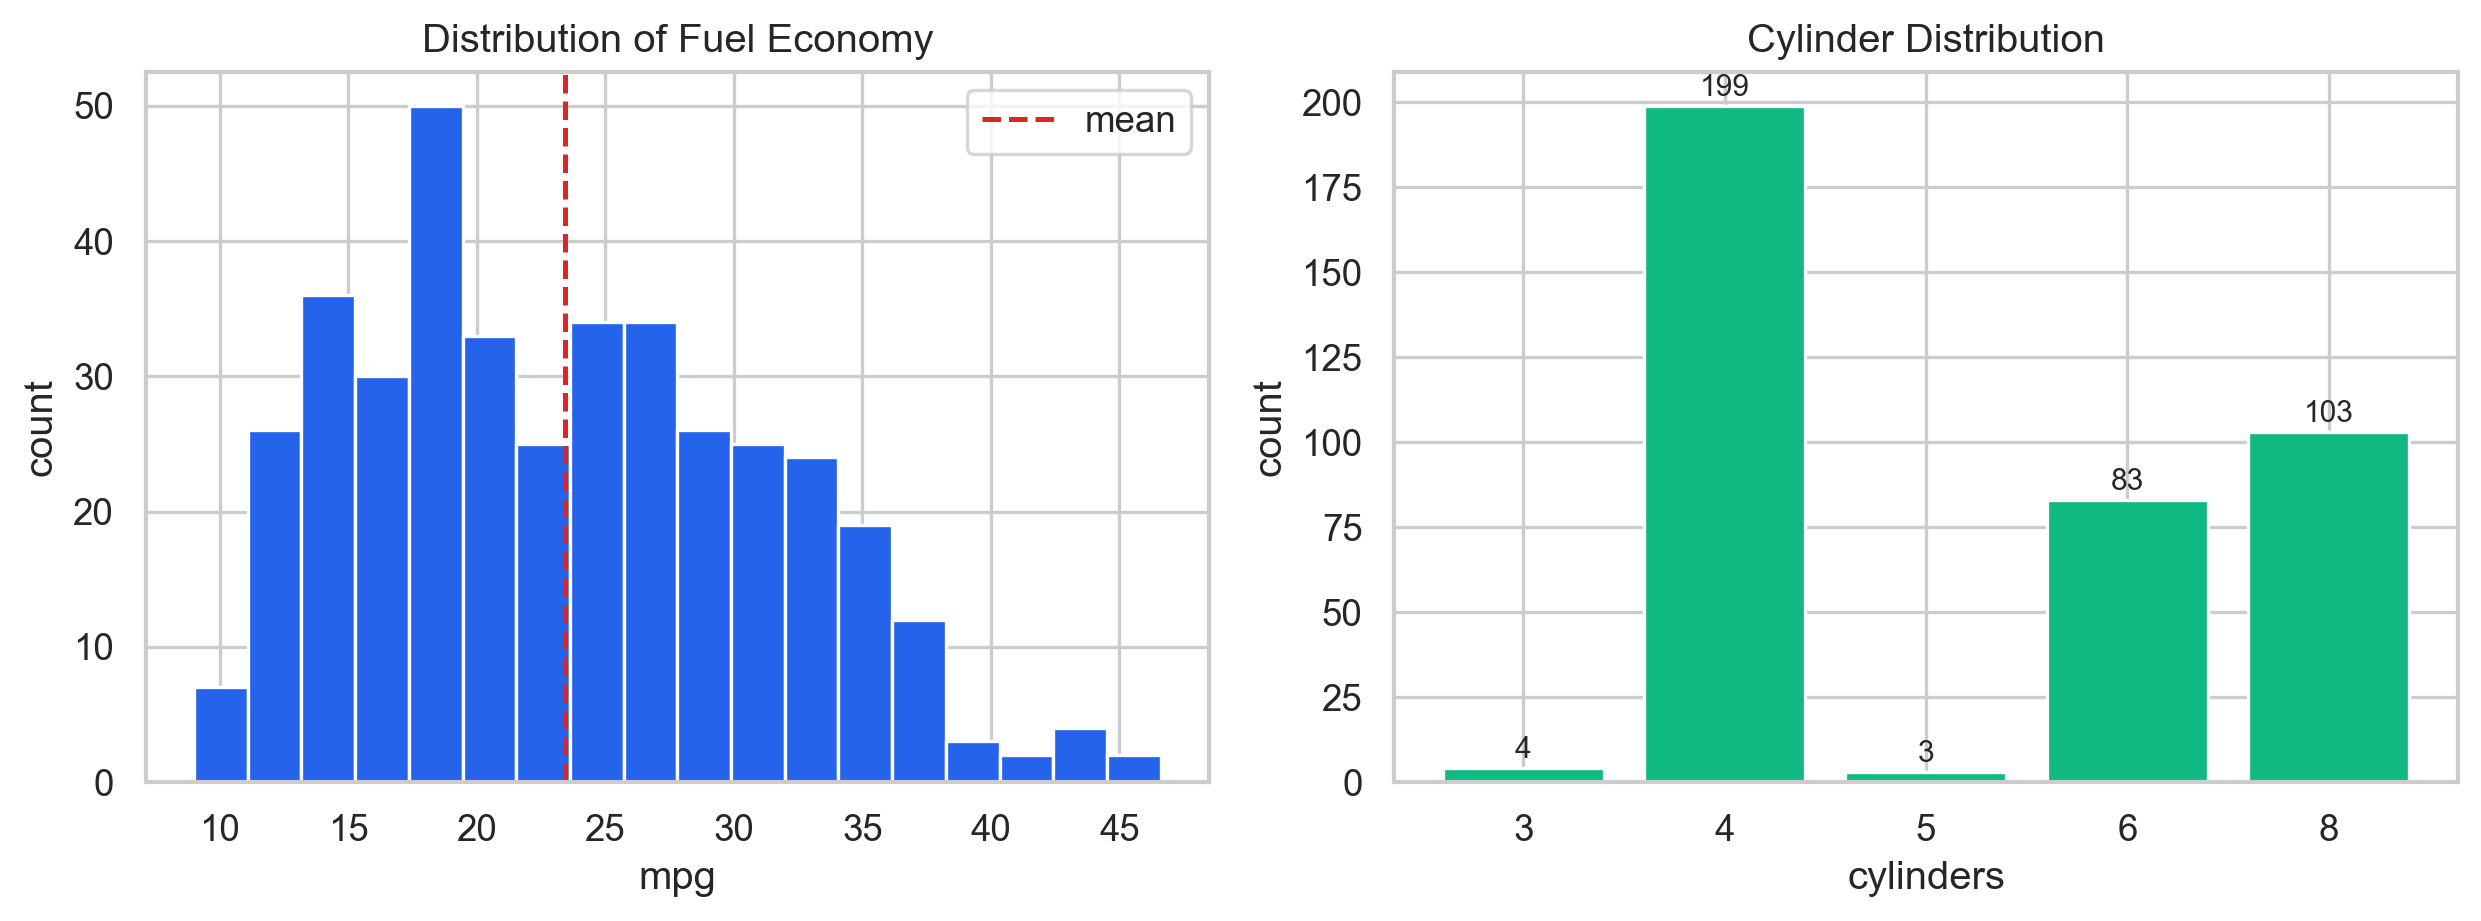
\includegraphics[width=0.9\linewidth]{figures/basic_distributions.png}
    \caption{燃油经济性与气缸数分布}
    \label{fig:basicdist}
\end{figure}

从图 \ref{fig:basicdist} 可见，\texttt{mpg} 分布范围较宽，四缸汽车数量最多。数值特征相关性热力图见图 \ref{fig:corr}。排量、气缸数、马力和重量之间具有较强正相关，而这些动力与尺寸指标均与 \texttt{mpg} 呈明显负相关。例如，重量与燃油经济性的相关系数约为 $-0.83$，说明重型车辆通常耗油更多。这种成组相关关系意味着汽车样本可能沿“轻量节能”和“重型高功率”方向形成自然结构。

\begin{figure}[H]
    \centering
    
\includegraphics[width=0.82\linewidth]{figures/correlation_heatmap.png}
    \caption{汽车数值特征相关性热力图}
    \label{fig:corr}
\end{figure}

图 \ref{fig:originmpg} 进一步展示生产地、重量与燃油经济性的关系。欧洲车和日本车整体更集中在轻量、高 mpg 区域，美国车覆盖范围更广，并包含较多重量大、燃油经济性低的车型。生产地可能与车型设计取向有关，但生产地本质上是名义类别，不能直接假设“日本与欧洲的距离小于日本与美国”。因此实验将 \texttt{origin} 进行 One-Hot 编码。

\begin{figure}[H]
    \centering
    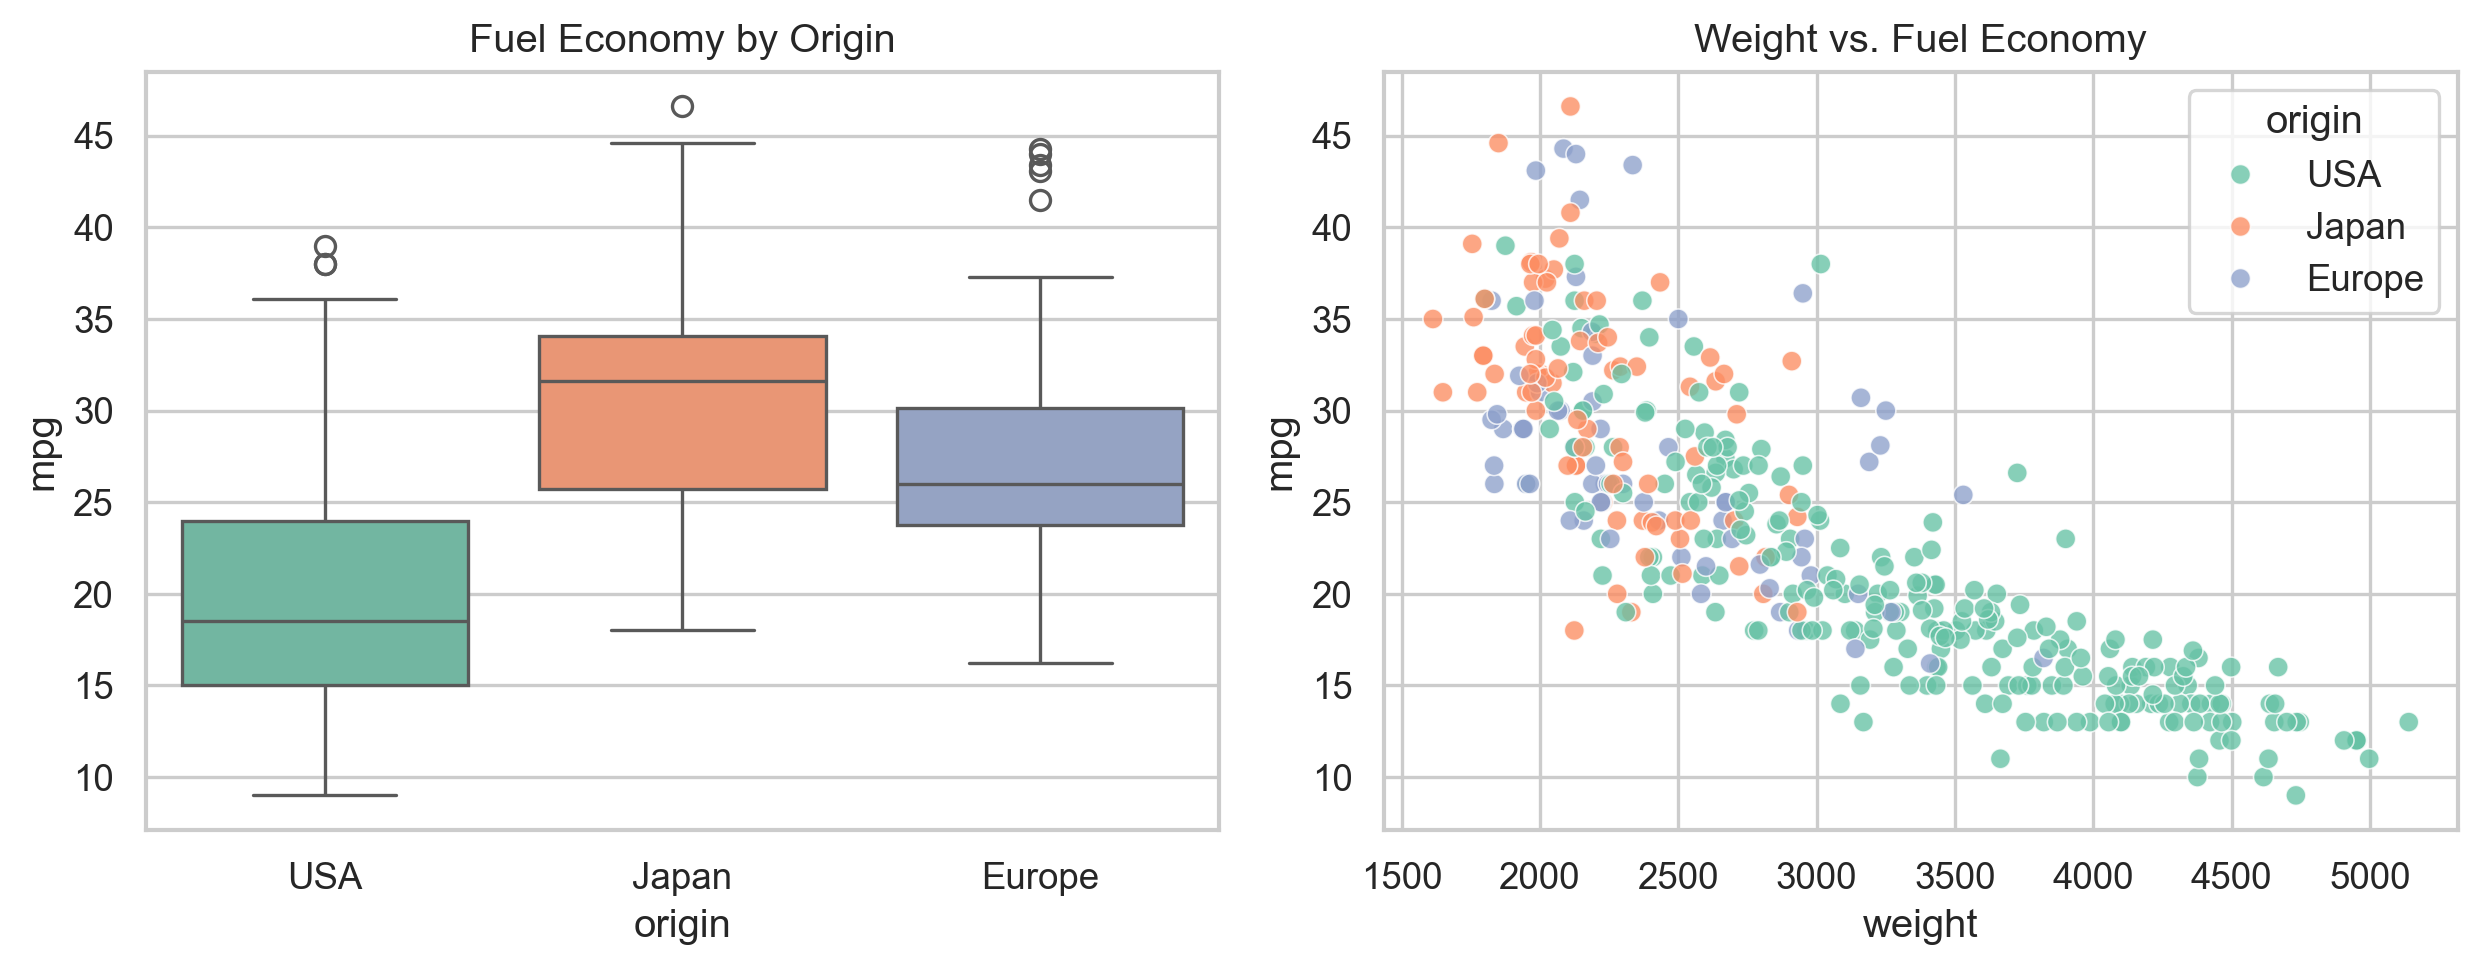
\includegraphics[width=0.9\linewidth]{figures/origin_and_weight_mpg.png}
    \caption{不同生产地的燃油经济性及重量--mpg关系}
    \label{fig:originmpg}
\end{figure}

\subsection{算法实现}

实验程序使用 \texttt{pandas} 读取和整理数据，使用 \texttt{scikit-learn} 完成预处理、聚类、指标评价和 PCA 降维，使用 \texttt{matplotlib} 与 \texttt{seaborn} 绘图。具体流程如下：

\begin{enumerate}
    \item 读取 \texttt{数据集.csv}，检查字段、数据类型、缺失值、重复值和描述性统计。
    \item 保存前 10 行数据、字段类型、缺失值统计、描述性统计、生产地分布和气缸数分布。
    \item 绘制燃油经济性分布、气缸数分布、相关性热力图，以及生产地、重量和 mpg 的关系图。
    \item 对 \texttt{mpg}、\texttt{cylinders}、\texttt{displacement}、\texttt{horsepower}、\texttt{weight}、\texttt{acceleration} 和 \texttt{year} 使用 Z-score 标准化；对 \texttt{origin} 使用 One-Hot 编码。预处理后共有 10 个输入维度。
    \item 对 K-Means 扫描 $K=2,\ldots,8$，记录簇内平方和、轮廓系数、Calinski--Harabasz 指数、Davies--Bouldin 指数和簇规模。
    \item 在选定的聚类数下比较 K-Means、Ward 层次聚类和 Gaussian Mixture；同时在参数网格中搜索 DBSCAN，并记录噪声比例。
    \item 对 K-Means 使用 20 组不同随机种子重新训练，以 ARI 检查结果稳定性。
    \item 选择内部指标表现较好的模型作为最终模型，输出聚类后的完整数据、各簇规模、原始特征均值、生产地比例和气缸数比例。
    \item 使用 PCA 二维投影、轮廓图、标准化聚类画像雷达图和重量--mpg 散点图解释聚类结果。
\end{enumerate}

完整 Python 程序见附录。

\section{实验结果与可扩展内容}

\subsection{实验结果}

K-Means 聚类数扫描结果见图 \ref{fig:kselect} 和表 \ref{tab:kselect}。当 $K$ 从 2 增加至 3 时，簇内平方和从 1447.46 降至 1087.16，之后仍会继续下降，这是增加聚类数的自然结果。但 $K=2$ 的轮廓系数最高，为 0.4347，同时 Davies--Bouldin 指数最低，为 0.8318；从 $K=3$ 开始，轮廓系数明显下降。因此，本实验选择两个主要汽车款式。

\begin{figure}[H]
    \centering
    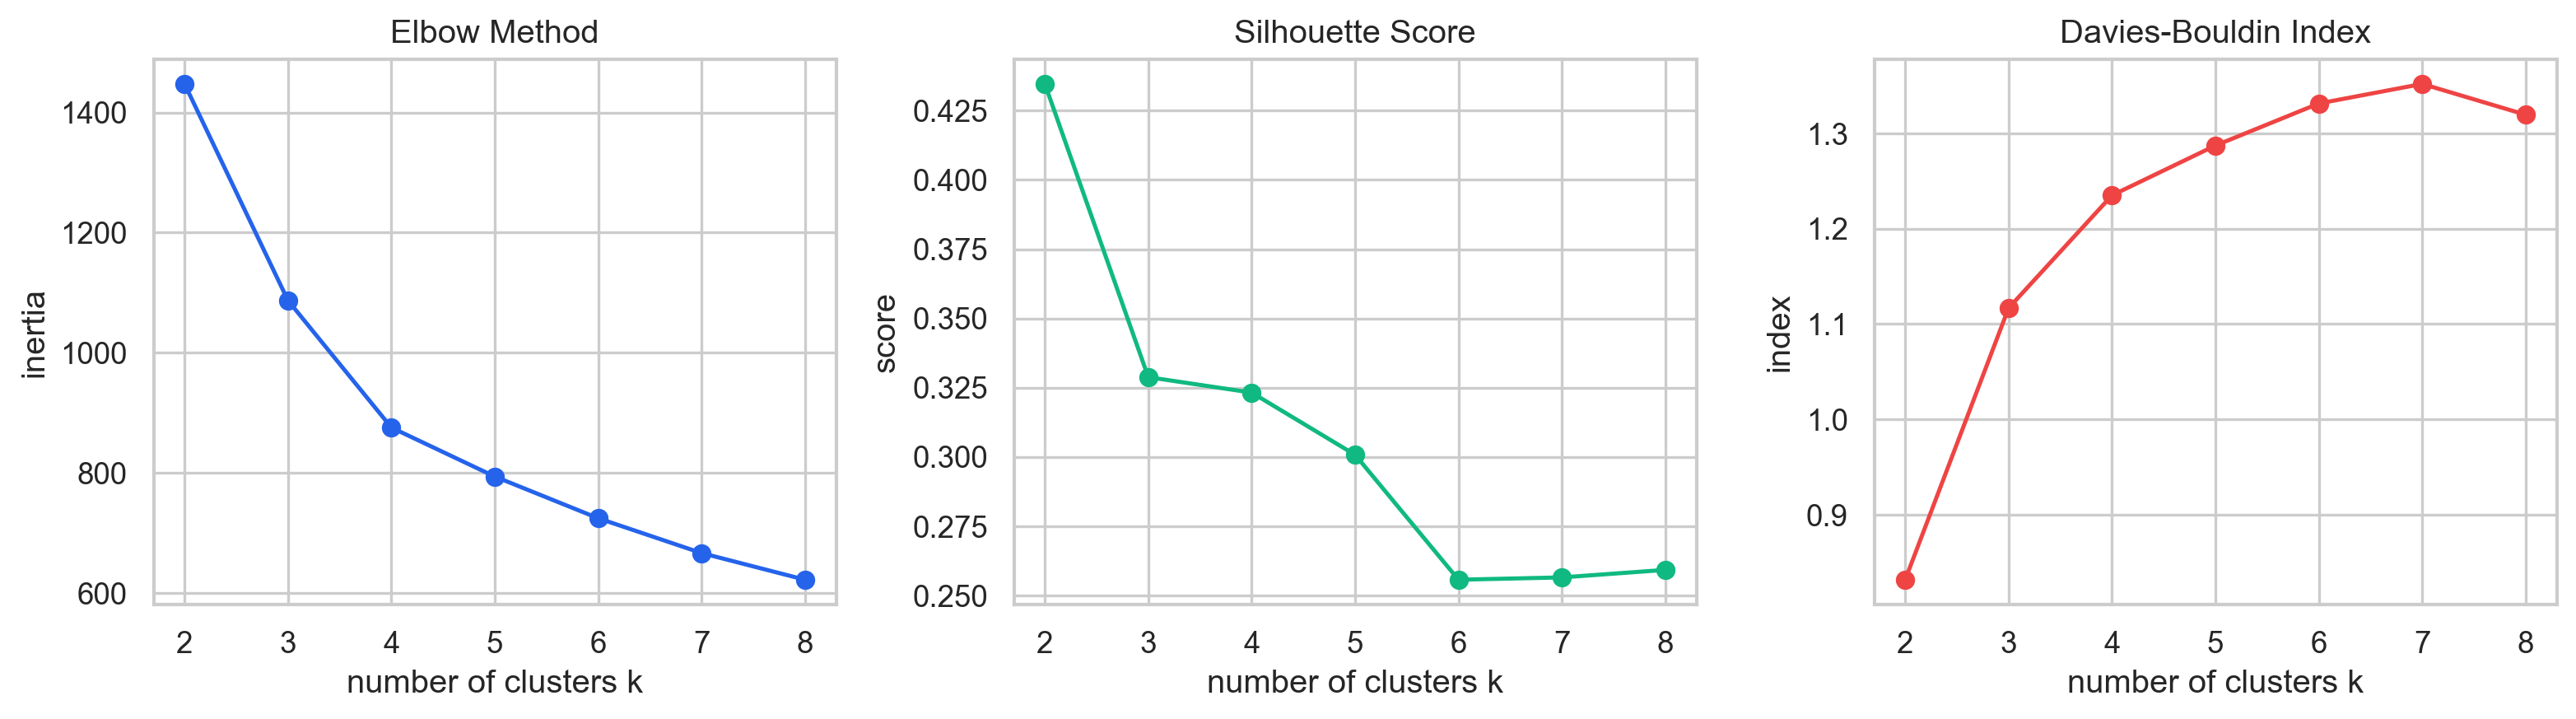
\includegraphics[width=0.98\linewidth]{figures/kmeans_k_selection.png}
    \caption{K-Means聚类数选择结果}
    \label{fig:kselect}
\end{figure}

\begin{table}[H]
\centering
\caption{不同聚类数下的K-Means内部评价指标}
\label{tab:kselect}
\small
\begin{tabular}{rrrrr}
\toprule
$K$ & 簇内平方和 & 轮廓系数 & Calinski--Harabasz & Davies--Bouldin\\
\midrule
2 & 1447.46 & 0.4347 & 406.23 & 0.8318\\
3 & 1087.16 & 0.3288 & 334.19 & 1.1167\\
4 & 875.71 & 0.3232 & 307.11 & 1.2349\\
5 & 794.19 & 0.3008 & 263.25 & 1.2872\\
6 & 724.82 & 0.2556 & 237.55 & 1.3313\\
7 & 666.87 & 0.2565 & 220.18 & 1.3518\\
8 & 622.52 & 0.2592 & 205.56 & 1.3195\\
\bottomrule
\end{tabular}
\end{table}

表 \ref{tab:modelcompare} 给出了不同算法的比较。Ward 层次聚类的轮廓系数最高，为 0.4558，Davies--Bouldin 指数也最低，为 0.7469，因此将其作为最终聚类模型。K-Means 的轮廓系数为 0.4347，虽然略低于层次聚类，但 Calinski--Harabasz 指数最高；两种算法的 ARI 为 0.7711，说明它们对汽车总体结构的判断较为一致。Gaussian Mixture 的轮廓系数仅为 0.2343。DBSCAN 在最优搜索参数 \texttt{eps=0.9}、\texttt{min\_samples=10} 下形成 6 个簇，但将 33.16\% 的样本判为噪声，其轮廓系数只在非噪声样本上计算，不能与其余算法完全等价比较。

\begin{table}[H]
\centering
\caption{不同聚类算法的内部评价结果}
\label{tab:modelcompare}
\small
\begin{tabular}{lrrrrr}
\toprule
算法 & 簇数 & 噪声比例 & 轮廓系数 & Davies--Bouldin & 与K-Means的ARI\\
\midrule
Ward层次聚类 & 2 & 0 & 0.4558 & 0.7469 & 0.7711\\
K-Means & 2 & 0 & 0.4347 & 0.8318 & 1.0000\\
DBSCAN & 6 & 0.3316 & 0.4138 & 0.9594 & 0.2665\\
Gaussian Mixture & 2 & 0 & 0.2343 & 1.3791 & 0.1332\\
\bottomrule
\end{tabular}
\end{table}

此外，K-Means 在 20 组不同随机种子下与参考结果的平均 ARI 为 0.9927，标准差为 0.0099，最小值仍达到 0.9792，说明两类结构具有较高稳定性。尽管最终模型采用不依赖随机初始化的 Ward 层次聚类，K-Means 稳定性实验仍从另一角度验证了数据中的主要分组不是由一次随机初始化偶然产生的。

最终模型将 392 辆汽车划分为两类：292 辆“节能轻量型”，占 74.49\%；100 辆“高功率重型”，占 25.51\%。两类原始特征均值见表 \ref{tab:profiles}。

\begin{table}[H]
\centering
\caption{最终聚类的汽车款式画像}
\label{tab:profiles}
\small
\begin{tabular}{lrrrrrrrr}
\toprule
类别 & mpg & 气缸 & 排量 & 马力 & 重量 & 加速时间 & 年份 & 生产地均值\\
\midrule
节能轻量型 & 26.45 & 4.61 & 142.68 & 85.32 & 2585.81 & 16.51 & 76.75 & 1.77\\
高功率重型 & 14.68 & 7.98 & 345.47 & 160.40 & 4121.56 & 12.70 & 73.74 & 1.00\\
\bottomrule
\end{tabular}
\end{table}

“节能轻量型”平均燃油经济性为 26.45 mpg，平均重量为 2585.81，平均马力为 85.32；其中 68.15\% 为四缸车，28.08\% 为六缸车，生产地构成为美国 49.66\%、欧洲 23.29\%、日本 27.05\%。这一类车型整体较轻、排量和马力较小、生产年份较新，燃油经济性更好。

“高功率重型”平均燃油经济性仅为 14.68 mpg，平均重量达到 4121.56，平均马力为 160.40；其中 99\% 为八缸车，1\% 为六缸车，并且全部来自美国。该类车辆平均从 0 加速到 60 mph 的时间为 12.70，低于节能轻量型的 16.51，说明其虽然车身更重、油耗更高，但动力与加速性能更强。生产年份均值为 73.74，也表明该类车型更集中于较早年代。

\begin{figure}[H]
    \centering
    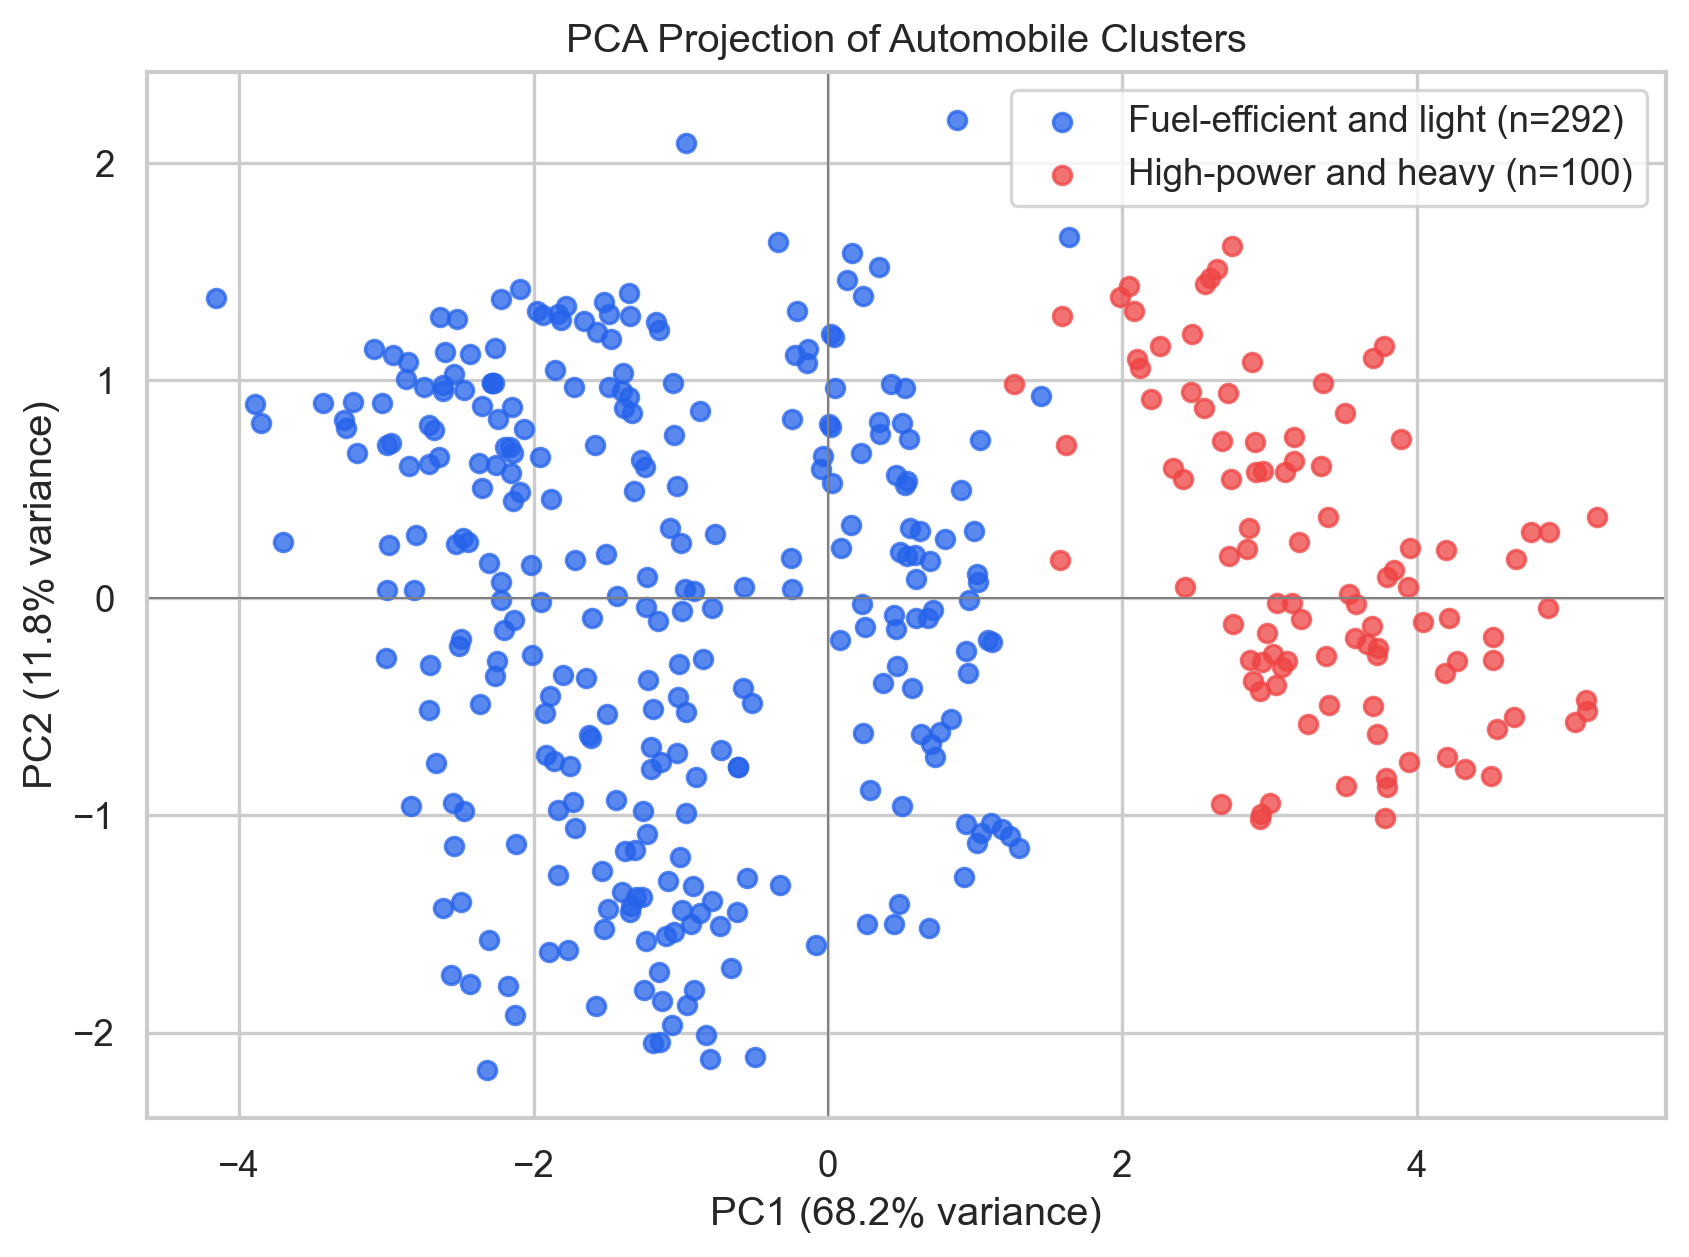
\includegraphics[width=0.88\linewidth]{figures/pca_clusters.png}
    \caption{最终聚类结果的PCA二维投影}
    \label{fig:pca}
\end{figure}

图 \ref{fig:pca} 中，第一主成分解释 68.2\% 的方差，第二主成分解释 11.8\%，两者合计解释 79.9\% 的信息。两类汽车主要沿第一主成分方向分离，高功率重型车辆集中在右侧，节能轻量型车辆分布在左侧。少量样本位于边界附近，说明中等重量、中等排量的汽车仍具有连续过渡，而不是完全孤立的两个群体。

\begin{figure}[H]
    \centering
    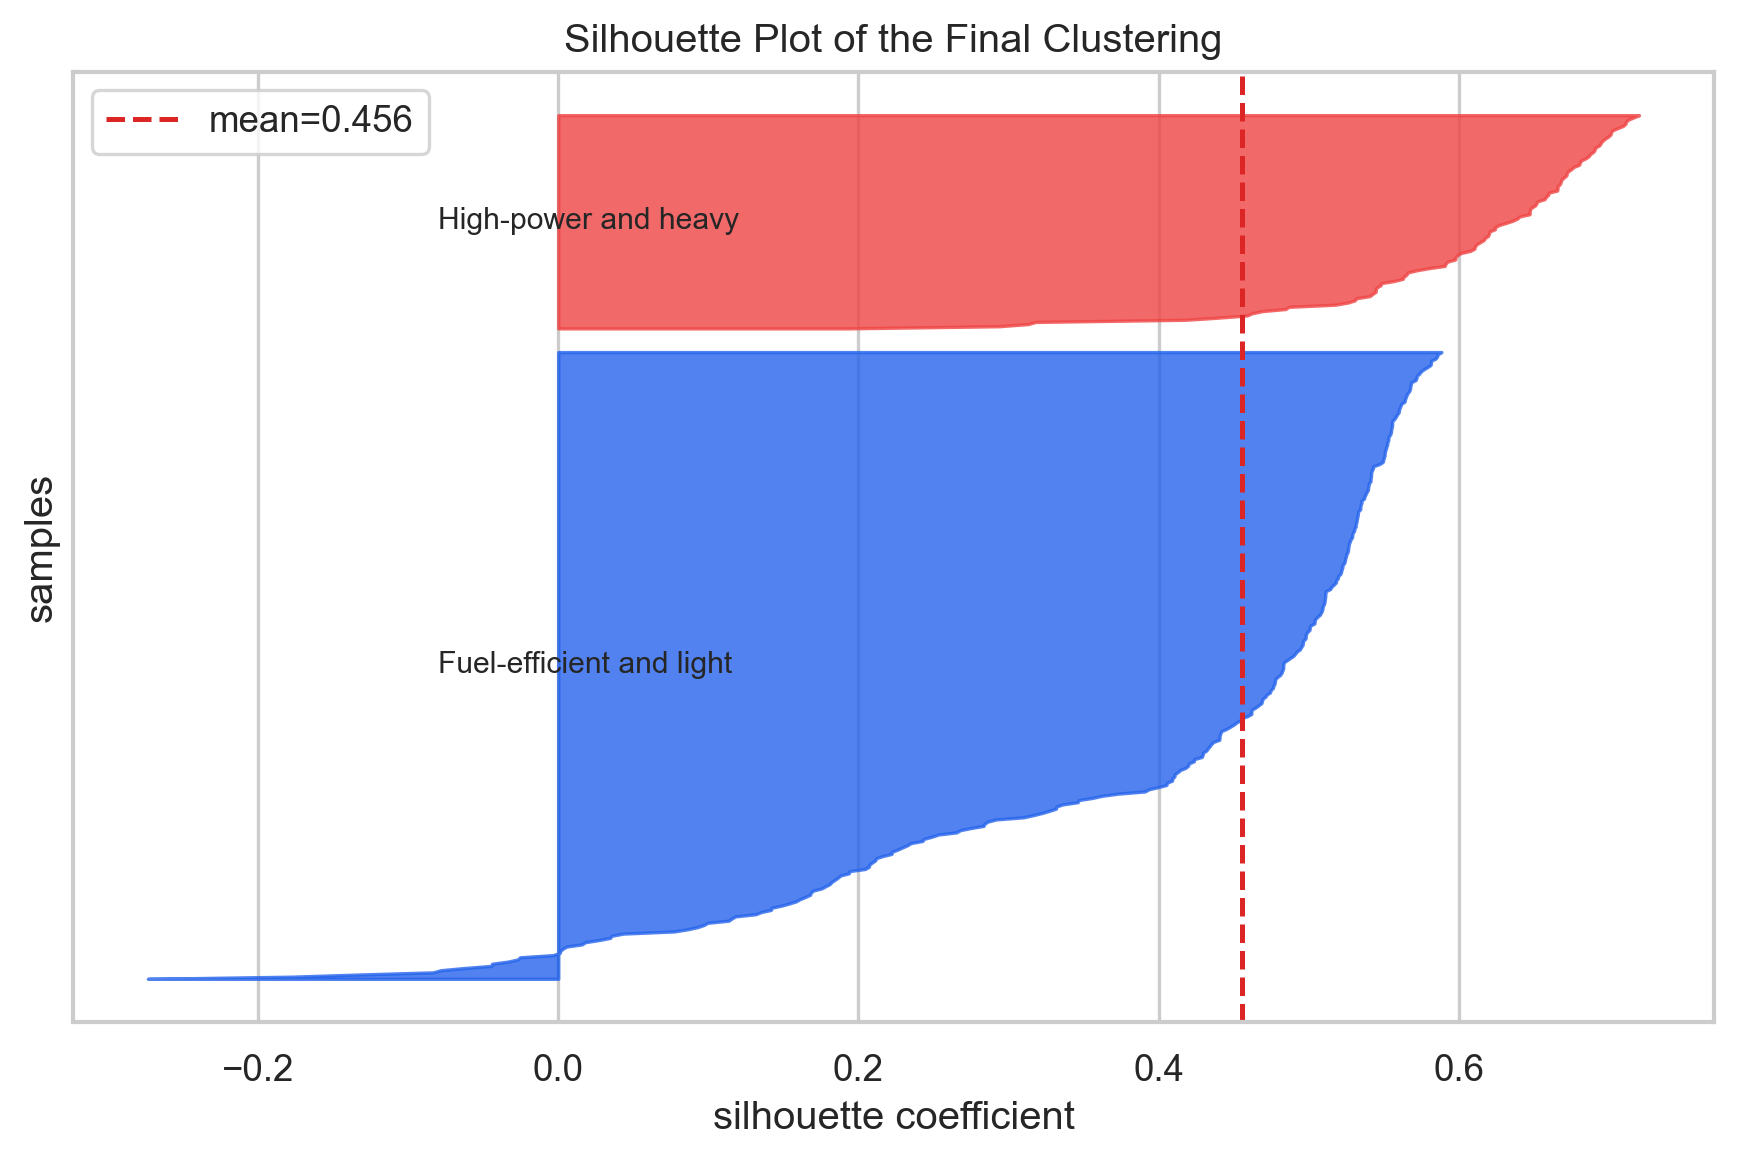
\includegraphics[width=0.76\linewidth]{figures/silhouette_plot.png}
    \caption{最终层次聚类的轮廓系数分布}
    \label{fig:silhouette}
\end{figure}

轮廓图见图 \ref{fig:silhouette}。平均轮廓系数为 0.4558，大多数样本轮廓系数为正，说明总体分组较合理；少量靠近零或为负的样本多处于两类车型的过渡区域。对于真实汽车数据，这种边界模糊是合理的，因为动力、重量和油耗本身是连续变化的。

\begin{figure}[H]
    \centering
    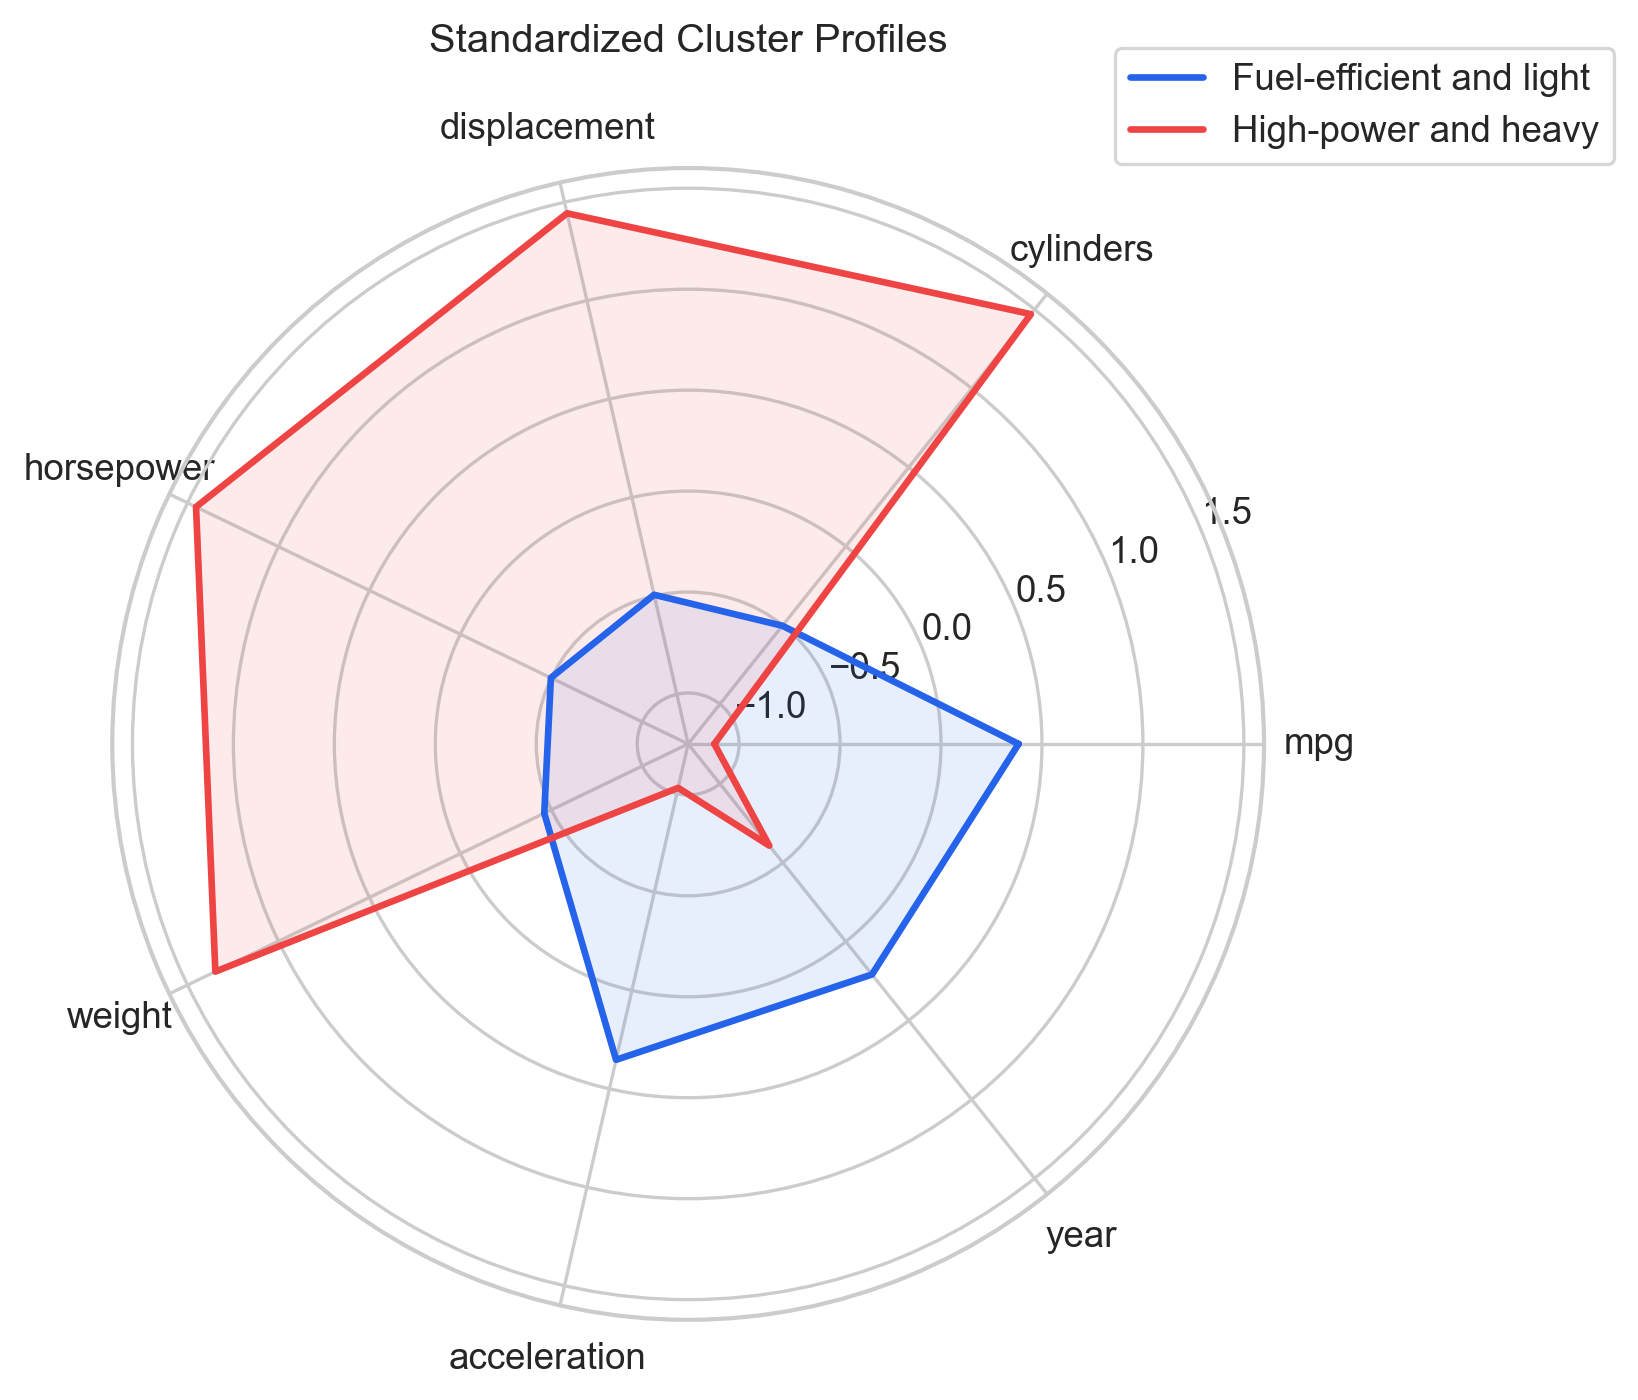
\includegraphics[width=0.76\linewidth]{figures/cluster_profile_radar.png}
    \caption{两类汽车的标准化特征画像}
    \label{fig:radar}
\end{figure}

图 \ref{fig:radar} 将各簇均值相对于全体数据进行标准化。高功率重型车辆在气缸数、排量、马力和重量上明显高于总体均值，在 mpg、年份和加速时间数值上低于总体均值；节能轻量型则呈现相反模式。该结果与相关性分析一致，表明聚类主要捕捉了车辆尺寸、动力和燃油经济性之间的综合差异。

\begin{figure}[H]
    \centering
    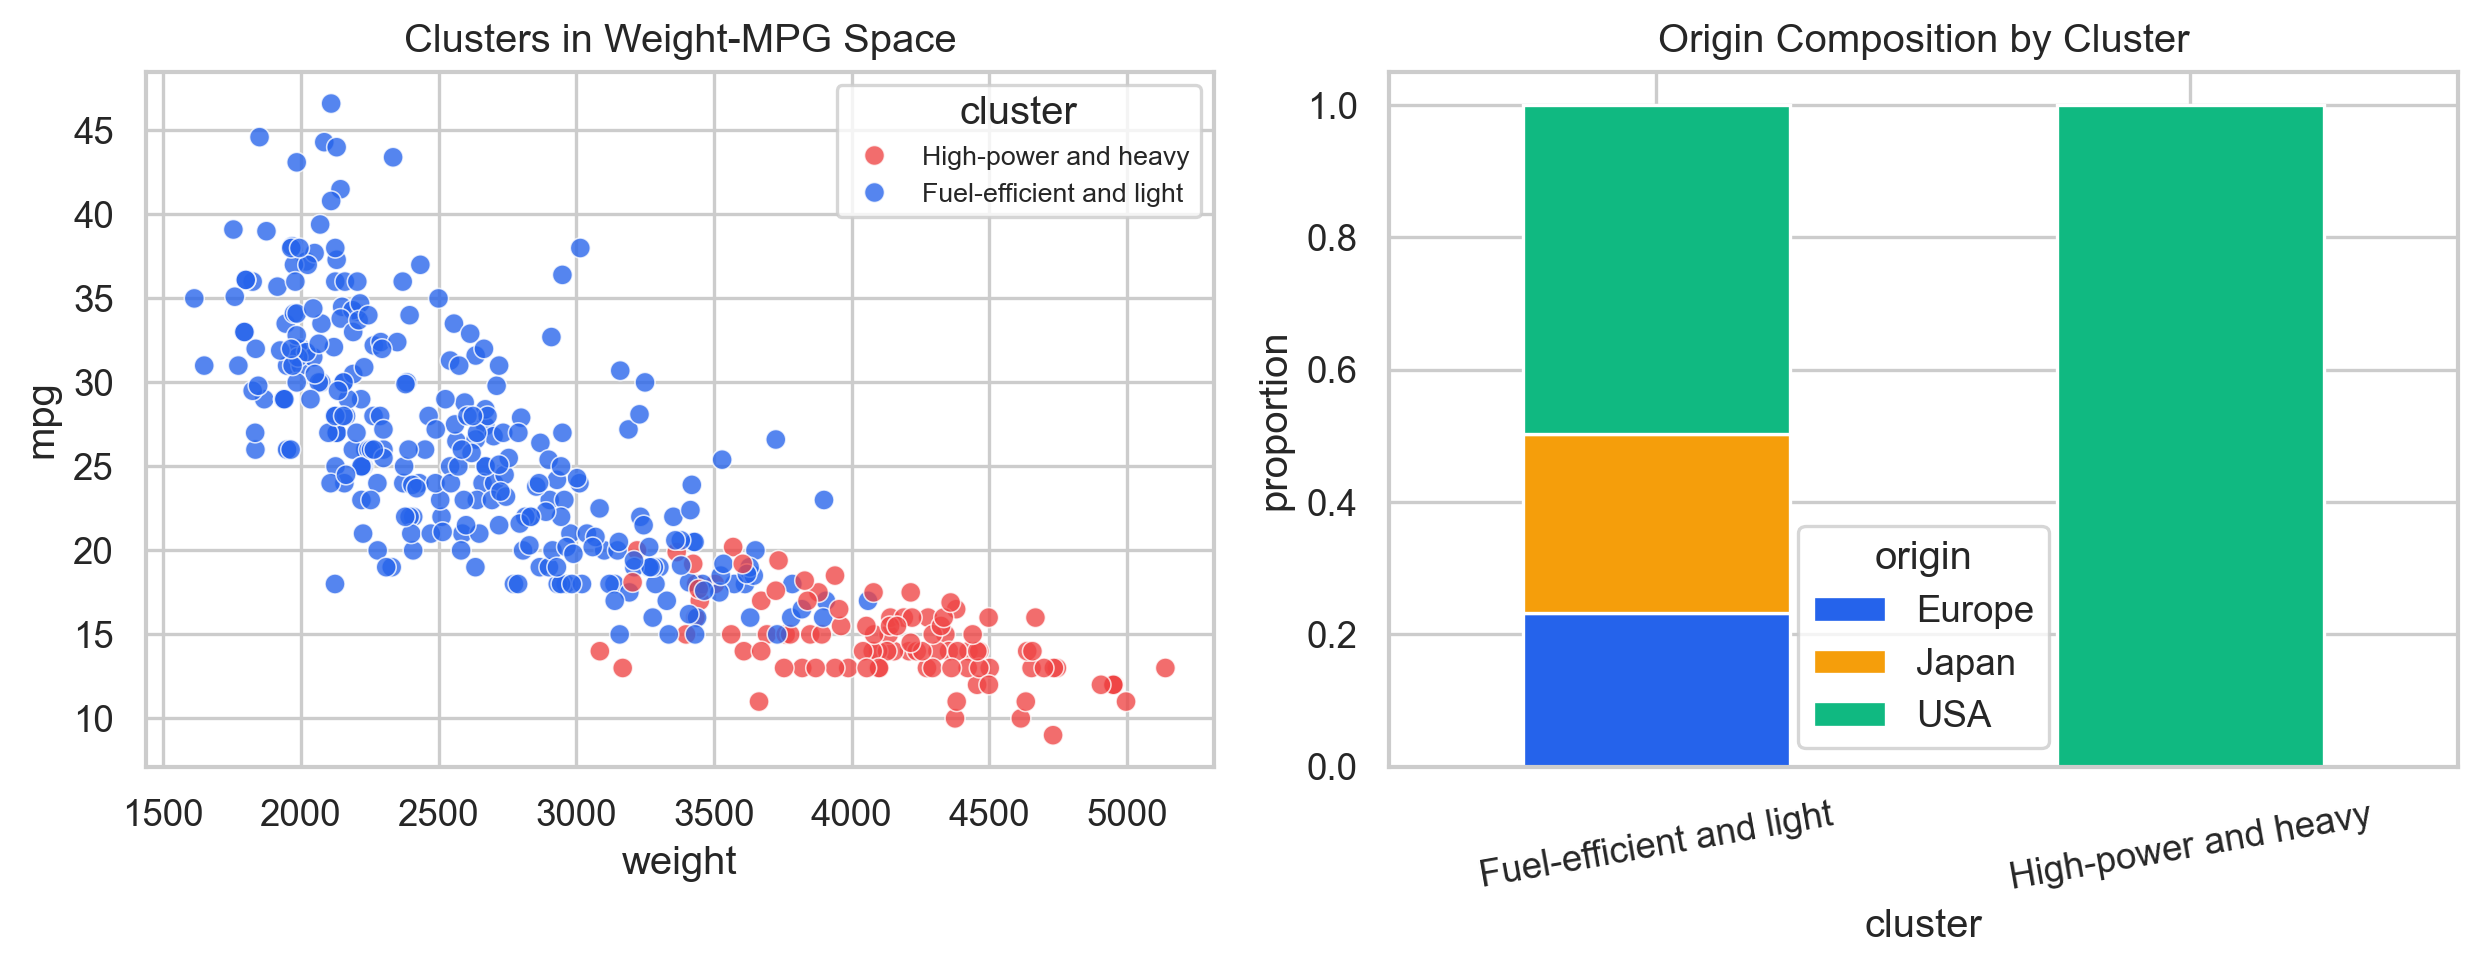
\includegraphics[width=0.94\linewidth]{figures/cluster_interpretation.png}
    \caption{重量--mpg空间中的聚类及各类生产地构成}
    \label{fig:interpretation}
\end{figure}

图 \ref{fig:interpretation} 左图显示，高功率重型车辆主要集中在高重量、低 mpg 区域；右图则显示该类车型全部来自美国，而节能轻量型同时包含美国、欧洲和日本车型。这并不表示“生产地决定类别”，因为聚类同时利用了所有参数，但它揭示了本数据所覆盖年代内不同地区车型设计取向的统计差异。

\subsection{参数调优及可扩展内容}

本实验通过 $K=2,\ldots,8$ 的网格扫描选择 K-Means 聚类数，并对 DBSCAN 的 \texttt{eps} 和 \texttt{min\_samples} 进行组合搜索。结果表明，继续增加 K 虽然可以降低簇内平方和，但会使轮廓系数下降、Davies--Bouldin 指数上升，因此不应仅凭簇内平方和选择更复杂的划分。两个主要簇能够提供最清晰、最稳定的宏观车型分组。

若需要更细粒度的市场细分，可以在“节能轻量型”内部再次聚类，将小型经济车、中型均衡车和不同生产地车型进一步区分。这种分层聚类思路比直接在全体数据上强制设置较大的 K 更容易解释。还可以使用 UMAP 或 t-SNE 辅助观察非线性结构，但这些降维方法对参数和随机种子较敏感，不应单独作为确定聚类数的依据。

在特征处理方面，本实验对 \texttt{origin} 使用 One-Hot 编码，避免把生产地当作有序数值。未来可以根据实际任务调整特征权重：如果更关注机械结构，可降低生产地和年份的影响；如果更关注消费市场，可加入价格、车身尺寸、品牌、维护成本和安全配置等变量。还可以使用 Gower 距离或 k-prototypes 等适合混合数据类型的算法，进一步减少数值特征与类别特征共同建模时的距离偏差。

\section{讨论与结论}

\subsection{结果讨论}

实验结果表明，Auto 数据集最显著的结构是“节能轻量型”与“高功率重型”的二分。两个类别不仅在重量和 mpg 上明显不同，在气缸数、排量、马力、加速时间和生产年份上也形成一致差异。这说明聚类结果并非由某一个字段单独决定，而是由多个相互关联的汽车参数共同形成。

Ward 层次聚类的平均轮廓系数为 0.4558，略优于 K-Means 的 0.4347。K-Means 与层次聚类之间的 ARI 为 0.7711，同时 K-Means 的随机种子稳定性接近 1，说明两个算法虽然对部分边界车辆的划分不同，但都识别出了同一主导结构。Gaussian Mixture 的表现较弱，可能是因为标准化后的汽车数据并不满足简单的两个完整高斯分布假设。DBSCAN 则将较多样本视为噪声，说明该数据更接近连续变化的椭球状群体，而不是由高密度核心和稀疏间隔组成的形状。

需要注意的是，聚类类别名称是根据特征均值进行的人工解释，并非数据集中原有标签。“节能轻量型”和“高功率重型”表示统计意义上的相似组，不等同于严格的汽车行业级别。生产地构成也只反映 1970 至 1982 年、该数据样本范围内的规律，不能直接推广到当前汽车市场。

\subsection{结论总结}

本次实验完成了基于 ISLR Auto 数据集的汽车款式聚类分析。实验对 7 个数值特征进行标准化，对生产地进行 One-Hot 编码，并使用多种内部指标选择聚类数。结果显示，$K=2$ 时 K-Means 的轮廓系数最高且 Davies--Bouldin 指数最低，说明两类划分最清晰。

在算法比较中，Ward 层次聚类取得 0.4558 的最高轮廓系数，因此被选为最终模型。最终得到 292 辆节能轻量型汽车和 100 辆高功率重型汽车。前者具有较高 mpg、较低重量、较小排量和较新年份，来源更加多样；后者几乎全部为美国八缸车，重量、排量和马力明显更高，但燃油经济性较低。

综合来看，聚类分析能够将多个汽车参数压缩为直观的车型分组，帮助理解复杂数据中的总体结构。完整流程涵盖数据检查、探索性分析、特征编码、标准化、聚类数选择、算法比较、稳定性验证、降维可视化和聚类解释，体现了无监督学习任务中“先保证距离合理，再评价结构，最后结合业务含义解释”的基本思路。

\section{心得体会与思考}

\subsection{个人心得}

通过本次实验，我对监督学习和无监督学习的差异有了更直观的认识。分类任务有真实标签，可以直接计算准确率；聚类任务没有标准答案，需要同时观察内部评价指标、二维可视化和各簇特征画像。仅得到一个聚类编号并不能说明结果有意义，必须进一步回答每个簇包含哪些样本、各项参数有什么差异，以及这些差异是否符合实际常识。

我也体会到数据预处理对聚类尤其重要。汽车重量可达到数千，生产地只有 1、2、3，如果直接计算欧氏距离，重量会在距离中占据过大作用，而生产地编码还会引入不存在的顺序关系。通过标准化和 One-Hot 编码，各项特征才能在较合理的尺度上共同参与聚类。

\subsection{启发与思考}

聚类数并不是越多越好。更多的簇一定会降低簇内平方和，但不一定能形成更清晰、更稳定、更容易解释的结构。本实验中 $K=2$ 的轮廓系数明显高于 $K=3$ 至 $K=8$，说明数据首先呈现的是两种宏观设计取向。若实际应用需要更细分类，应在已有大类内部继续细分，并结合业务目标确定粒度，而不是机械地追求更多类别。

此外，PCA 图让我看到聚类边界并非绝对分离。部分车辆位于两类之间，说明汽车参数存在连续过渡。实际决策中可以进一步计算样本到簇中心的距离或使用概率聚类，给出“典型程度”或不确定性，不应把每辆车视为绝对固定的款式。

\clearpage
\section{附录}

\subsection*{算法代码及其注释}
\addcontentsline{toc}{subsection}{算法代码及其注释}

\VerbatimInput[breaklines,breakanywhere,fontsize=\small,frame=single,rulecolor=\color{gray!45}]{report_code.py}

\clearpage
\subsection*{关键运行结果汇总}
\addcontentsline{toc}{subsection}{关键运行结果汇总}

\begin{CodeBlock}
数据规模: 392 行, 8 列
缺失值: 0
重复记录: 0
预处理后特征维度: 10

最优主要聚类数: 2
最终模型: Agglomerative_Ward
最终轮廓系数: 0.455824

聚类规模:
Fuel-efficient and light: 292
High-power and heavy: 100

K-Means 20 组随机种子稳定性:
平均 ARI: 0.992732
标准差: 0.009904
最小 ARI: 0.979235

PCA 解释方差:
PC1: 68.19%
PC2: 11.76%
合计: 79.95%
\end{CodeBlock}

\end{document}
